%%
% The BIThesis Template for Bachelor Graduation Thesis
%
% 北京理工大学毕业设计(论文) —— 使用 XeLaTeX 编译
%
% Copyright 2021-2023 BITNP
%
% This work may be distributed and/or modified under the
% conditions of the LaTeX Project Public License, either version 1.3
% of this license or (at your option) any later version.
% The latest version of this license is in
%   http://www.latex-project.org/lppl.txt
% and version 1.3 or later is part of all distributions of LaTeX
% version 2005/12/01 or later.
%
% This work has the LPPL maintenance status `maintained'.
%
% The Current Maintainer of this work is Feng Kaiyu.
%
% Compile with: xelatex -> biber -> xelatex -> xelatex

% 开启盲审格式 blindPeerReview=true (如:[type=bachelor,blindPeerReview=true])

\documentclass[type=bachelor]{bithesis}

\BITSetup{
  cover = {
    % 在封面中载入有「北京理工大学」字样的图片,如无必要请勿改动。
    headerImage = images/header.png,
    % 在封面标题中使用思源黑体,使用此选项可以保证与 Word 封面标题的字体一致。
    xiheiFont = STXIHEI.TTF,
    %% 使用以下参数来自定义封面日期
    % date = 2022年6月,
  },
  info = {
    % 想要删除某项封面信息,直接删除该项即可。
    % 想要让某项封面信息留空(但是保留下划线),请设置为空字符串。
    % 如需要换行,则用 “\\” 符号分割。
    title = 基于深度学习的端到端多实例点云配准,
    titleEn = {Deep Learning Based End-To-End Multi-instance  Point Cloud Registration},
    school = \quad 自动化学院 \quad,
    major = 自动化,
    author = 杨润一,
    class = 06111902,
    studentId = 1120191211,
    supervisor = 由育阳,
    keywords = {点云配准; 多实例; 聚类; 对应聚类; 深度学习},
    keywordsEn = {Point Cloud Registration; Multi-instance; Clustering; Correspondence Clustering; Deep Learning},
    % 如果你的毕设为校外毕设,请将下面这一行语句解除注释(删除第一个百分号字符)并填写你的校外毕设导师名字
    % externalSupervisor = 左偏树,
  },
  style = {
    % 保持参考文献的缩进样式与 Word 模板一致。
    % 如果你不需要此样式,请将此行注释掉。
    bibliographyIndent = false,
  }
}

% 使用 listings 宏包进行代码块使用,并使用了预定义的样式,
% 你也可以选用自己的喜欢的其他宏包,如 minted;
% 然而由于 minted 依赖 Python 的 Pygments 库作为外部依赖,因此出于模板的简洁程度考虑,我们没有提供 minted 进行代码块书写的示例。
\usepackage{listings}

\usepackage[
  backend=biber,
  style=gb7714-2015,
  gbalign=gb7714-2015,
  gbnamefmt=lowercase,
  gbpub=false,
  doi=false,
  url=false,
  eprint=false,
  isbn=false,
]{biblatex}

% 参考文献引用文件位于 misc/ref.bib
\addbibresource{misc/ref.bib}


% 文档开始
\begin{document}

% 标题页面:如无特殊需要,本部分无需改动
\MakeCover

% 原创性声明:如无特殊需要,本部分无需改动
% 更改为 PDF 页面插入,如需要添加内容,可考虑先用 Word 制作再覆盖 misc/1_originality.pdf
% ====== 原创性声明(PDF 格式)======
\begin{blindPeerReview}
  
\includepdf{misc/1_originality.pdf}\newpage
\end{blindPeerReview}
% ====== 原创性声明(PDF 格式)======
% ====== 原创性声明(LaTeX 格式)======
% %%
% The BIThesis Template for Bachelor Graduation Thesis
%
% 北京理工大学毕业设计(论文)原创性声明模板 —— 使用 XeLaTeX 编译
%
% Copyright 2020-2023 BITNP
%
% This work may be distributed and/or modified under the
% conditions of the LaTeX Project Public License, either version 1.3
% of this license or (at your option) any later version.
% The latest version of this license is in
%   http://www.latex-project.org/lppl.txt
% and version 1.3 or later is part of all distributions of LaTeX
% version 2005/12/01 or later.
%
% This work has the LPPL maintenance status `maintained'.
%
% The Current Maintainer of this work is Feng Kaiyu.
%
% Compile with: xelatex -> biber -> xelatex -> xelatex
%
% 如无特殊需要,本页面无需更改

\MakeOriginality

% ====== 原创性声明(LaTeX 格式)======

% 前置页面定义
\frontmatter
% 摘要:在摘要相应的 TeX 文件处进行摘要部分的撰写
%%
% The BIThesis Template for Bachelor Graduation Thesis
%
% 北京理工大学毕业设计(论文)中英文摘要 —— 使用 XeLaTeX 编译
%
% Copyright 2020-2023 BITNP
%
% This work may be distributed and/or modified under the
% conditions of the LaTeX Project Public License, either version 1.3
% of this license or (at your option) any later version.
% The latest version of this license is in
%   http://www.latex-project.org/lppl.txt
% and version 1.3 or later is part of all distributions of LaTeX
% version 2005/12/01 or later.
%
% This work has the LPPL maintenance status `maintained'.
%  
% The Current Maintainer of this work is Feng Kaiyu.

% 中英文摘要章节
\begin{abstract}
    三维点云配准是点云处理中的一项基本任务,其在机械臂、自动驾驶、自主运动机器人、即时定位与地图构建(Simultaneous Localization and Mapping,SLAM)等众多基于视觉方法的应用中起着关键的作用。随着人工智能、元宇宙、自动驾驶等技术的兴起,将深度学习应用于点云配准的工作已经日趋成熟。目前大多数点云配准任务研究主要集中在成对配准上。然而,在实际应用中,目标场景可能包含多个重复实例,我们需要估计模板点云与目标点云中这些重复实例之间的多个刚性变换,也就是多实例点云配准。

    本文针对三维点云配准问题,特别是多实例点云配准,进行了深入研究。我们调研并整理了多实例点云配准的国内外研究现状,并总结了前人研究的优势和劣势。现有解决方案需要对大量假设进行采样以检测可能的实例并排除异常值,当实例和异常值的数量增加时,其鲁棒性和效率会显着降低。我们建议根据距离不变矩阵将噪声对应集直接分组到不同的簇中。通过聚类自动识别实例和异常值,达到稳健且快速表现。
    
    基于这一研究背景,我们提出了新的多实例点云配准架构,高效对应聚类的多实例点云配准 (ECC) 。分析聚类方法的点云配准,发现对于描述子的依赖性高,离群点比例高的时候效果会大大下降,所以我们提出了基于深度学习和聚类优化的多实例点云配准 (DMR),首先利用对比学习来学习输入推定对应关系的分布良好的深度表示。然后基于这些表示,我们提出了异常值修剪策略和聚类策略,以有效地删除异常值并将剩余的对应关系分配给正确的实例,达到了更好的效果。
    
    综上所述,我们的研究表明,基于深度学习的多实例点云配准方法在处理复杂的多实例点云配准问题上具有优秀的性能,提供了新的研究思路和方法。
    
\end{abstract}

% 英文摘要章节
\begin{abstractEn}
    Three-dimensional point cloud registration is a fundamental task in point cloud processing, which plays a crucial role in a wide range of vision-based applications such as robotic arms, autonomous driving, autonomous mobile robots, and Simultaneous Localization and Mapping (SLAM). With the rise of artificial intelligence, metaverse, autonomous driving, and other technologies, the application of deep learning to point cloud registration has become increasingly mature. Current research on point cloud registration mostly focuses on pairwise registration. However, in practical applications, the target scene may contain multiple repeated instances, and we need to estimate multiple rigid transformations between the template point cloud and these repeated instances in the target point cloud, that is, multi-instance point cloud registration.

    This paper conducts in-depth research on the problem of three-dimensional point cloud registration, especially multi-instance point cloud registration. We have surveyed and summarized the domestic and international research status of multi-instance point cloud registration and summarized the advantages and disadvantages of previous studies. Existing solutions require sampling a large number of hypotheses to detect possible instances and reject outliers, and their robustness and efficiency degrade significantly when the number of instances and outliers increases. We propose to directly group the noisy correspondence set into different clusters based on a distance invariance matrix. Through clustering, instances and outliers are automatically identified, achieving robust and fast performance.
    
    Based on this research background, we propose a new multi-instance point cloud registration framework, \textbf{E}fficient \textbf{C}orrespondence \textbf{C}lustering for Multi-instance Point Cloud Registration (\textbf{ECC}). After analyzing the point cloud registration of the clustering method, we find that the effect will drop significantly when it has high dependency on the descriptor and a high proportion of outliers. Therefore, we propose \textbf{D}eep Learning and Cluster Opimisation based \textbf{M}ulti-instance Point Cloud \textbf{R}egistration (\textbf{DMR}), which first uses contrastive learning to learn a good deep representation of the input estimation correspondence. Then, based on these representations, we propose an outlier pruning strategy and a clustering strategy to effectively remove outliers and allocate the remaining correspondences to the correct instances, achieving better results.
    
    In conclusion, our research shows that the deep learning-based multi-instance point cloud registration method has excellent performance in dealing with complex multi-instance point cloud registration problems and provides new research ideas and methods.
\end{abstractEn}


\MakeTOC

% 正文开始
\mainmatter

% 第一章
%%
% The BIThesis Template for Bachelor Paper Translation
%
% 北京理工大学毕业设计(论文) —— 使用 XeLaTeX 编译
%
% Copyright 2020-2023 BITNP
%
% This work may be distributed and/or modified under the
% conditions of the LaTeX Project Public License, either version 1.3
% of this license or (at your option) any later version.
% The latest version of this license is in
%   http://www.latex-project.org/lppl.txt
% and version 1.3 or later is part of all distributions of LaTeX
% version 2005/12/01 or later.
%
% This work has the LPPL maintenance status `maintained'.
%
% The Current Maintainer of this work is Feng Kaiyu.
%
% Compile with: xelatex -> biber -> xelatex -> xelatex
%%

% 第一章节

\chapter{引言}

三维点云配准\cite{TEASER, DCP, paulj1992method}主要关注在源点云和目标点云之间估计一个单一的变换。然而,我们有时可能希望在点云之间估计多个变换。例如,我们有一个物体的3D扫描,可能希望在目标点云中找到如图\ref{fig:problem}所示的同一物体在桌子上的姿态。这个问题,我们称之为多实例点云配准,文献中较少研究。这个问题,我们称之为多实例点云配准,文献中较少研究。将现有的点云配准方法扩展到解决这个问题并非易事。

主要的挑战是在嘈杂的对应关系集合中识别属于不同实例的对应点的不同簇。一种解决方案是采用3D物体检测器或将实例分割应用于目标点云。然后,通过常规的点云配准方法估计每个实例的姿态。然而,这种方法需要为特定对象或类别训练检测器或分割网络\cite{VoteNet, Occuseg},不适用于未知对象或任意3D扫描。

\begin{figure}[htbp]
  \centering
  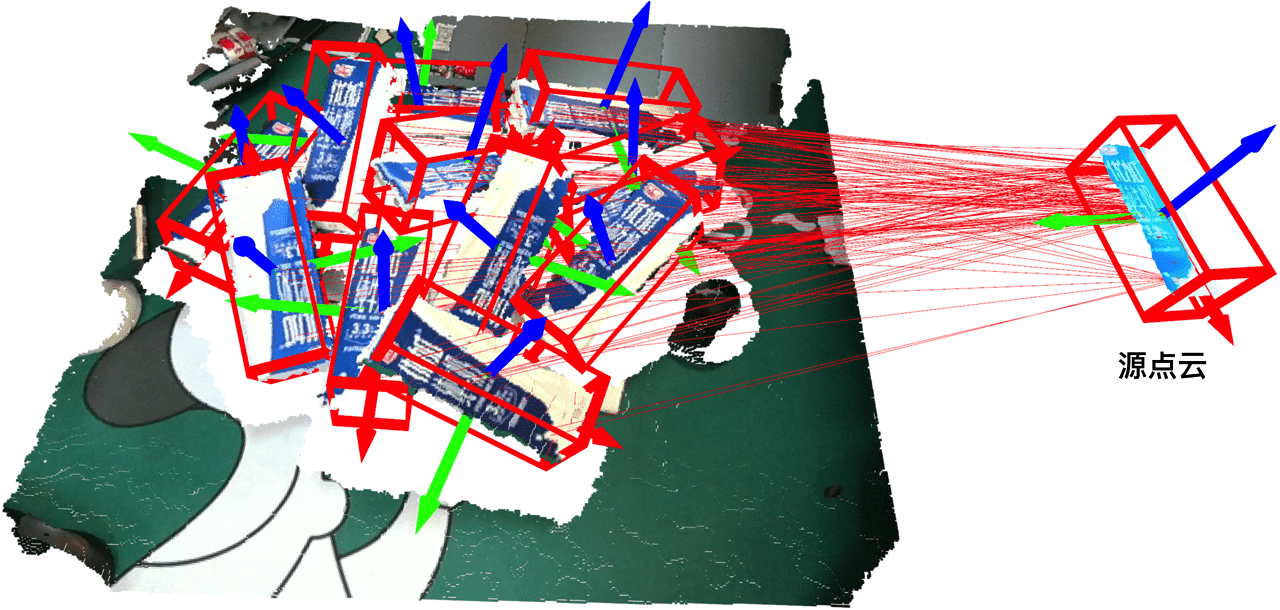
\includegraphics[width=0.8\textwidth]{images/problem.png}
  \caption{多实例点云配准:给定一个物体的源点云,多实例配准需要估计目标点云中每个物体的姿态。}
  \label{fig:problem} % label 用来在文中索引
  \vspace{-0.5in}
\end{figure}



另一种解决方案是通过多模型拟合\cite{Tlinkage, RPA, Coverage}或\cite{MCT, CONSAC, ProgressiveX2}。现有的多模型拟合方法依赖于采样有效的假设,当模型数量或异常值比例变高时,涉及大量的采样步骤,使得这些算法的效率和鲁棒性急剧下降。

在本文中,我们提出了一种鲁棒且高效的多实例三维配准问题解决方案。关键思想是根据距离不变性矩阵直接将对应点分组到不同的簇中。具体而言,在使用诸如D3Feat \cite{D3Feat}、PREDATOR \cite{PREDATOR}或SIFT \cite{lowe2004distinctive}等描述符进行特征匹配得到点对应关系之后,通过检查每对对应关系之间的距离一致性来构造矩阵。我们发现这个矩阵的行或列向量具有强大的表示能力,可以用于识别特定实例的对应关系集合。因此,我们应用了一种简单且高效的聚类算法将这些对应关系划分为团。通过将相似簇合并并重新分配簇id给每个对应关系,递归地进行几步细化聚类。最后,通过一个简单的排序策略自动识别每个实例的异常值和内点。



由于不需要耗时的假设采样,我们的方法具有很高的效率。我们在合成数据集和真实世界数据集上进行了广泛的实验。结果表明,我们的方法在准确性和鲁棒性方面表现明显优于现有方法,速度至少快10倍。总之,我们的贡献包括:
\begin{itemize}
\setlength{\itemsep}{-1pt}
\setlength{\parsep}{-2pt}
\item 我们提出了一种针对多实例点云配准问题的高效且鲁棒的解决方案,其在准确性、鲁棒性和速度方面都具有优越的性能。
\item 我们提出使用三个指标(平均命中召回率、平均命中精确度和平均命中F1)来全面评估多实例点云配准的性能。%据我们所知,尚未有针对这类评估的指标提出。
\item 我们的解决方案可以用于零样本检测3D物体,正如我们的真实世界测试所示。
\end{itemize}


% 在这里添加第二章、第三章……TeX 文件的引用
%%
% The BIThesis Template for Bachelor Paper Translation
%
% 北京理工大学毕业设计(论文) —— 使用 XeLaTeX 编译
%
% Copyright 2020-2023 BITNP
%
% This work may be distributed and/or modified under the
% conditions of the LaTeX Project Public License, either version 1.3
% of this license or (at your option) any later version.
% The latest version of this license is in
%   http://www.latex-project.org/lppl.txt
% and version 1.3 or later is part of all distributions of LaTeX
% version 2005/12/01 or later.
%
% This work has the LPPL maintenance status `maintained'.
%
% The Current Maintainer of this work is Feng Kaiyu.
%
% Compile with: xelatex -> biber -> xelatex -> xelatex
%%

% 第一章节

\chapter{相关工作}

\textbf{点云配准}可以分为三个阶段:点匹配、异常值剔除和姿态估计。大多数工作集中在前两个阶段,因为获得正确的点对应关系是成功配准的关键。点匹配通常依赖于特征,可以是手工设计的特征\cite{rusu2009fast, drost2010model},也可以是基于学习的特征\cite{3DMatch, PPFNet, 3DSmoothNet, FCGF, D3Feat}。尽管近期的结果显示,在某些基准测试中,后者优于手工设计的特征,但这些特征仍然无法实现完美匹配,因此仍然需要强大的异常值剔除机制。
RANSAC\cite{RANSAC}及其变体(\cite{GCRansac, NGRansac, LORansac})遵循假设-验证过程来剔除异常值。当存在许多异常值时,这类方法需要大量的采样步骤,耗时严重,而且仍可能无法获得正确的模型。GORE\cite{bustos2017guaranteed}和PMC\cite{parra2019practical}试图通过几何一致性检查来减少异常值。其他方法如FGR\cite{FGR}和TEASER\cite{TEASER}采用鲁棒估计器直接从噪声对应关系中解决变换问题。通过仔细处理每个子问题,TEASER\cite{TEASER}在鲁棒性和效率方面取得了令人印象深刻的性能。
还有一些基于学习的异常值剔除方法。DGR\cite{DGR}和3DRegNet\cite{3DRegNet}将异常值剔除视为二分类问题,并预测每个对应关系的内点概率。PointDSC\cite{PointDSC}进一步将空间一致性嵌入到特征学习中,以便更好地训练内点分类器。
最近,一系列工作(如PointNetLK\cite{PointNetLK},FMR\cite{FMR},DCP\cite{DCP},PRNet\cite{PRNet},RPMNet\cite{RPMNet})尝试将端到端学习应用于解决配准问题。它们在性能方面也表现出色,特别是在低重叠情况下\cite{PREDATOR}。

现有的点云配准方法主要关注一对一配准问题,即估计两个点云之间的单一变换。然而,将源点云与目标点云中的多个实例对齐的多实例配准问题则研究较少。这个任务与多路配准\cite{choi2015robust}不同,后者的目标是通过成对配准\cite{FGR}\cite{DGR}从多个片段生成全局一致的重建。多实例配准需要不仅从噪声对应关系中剔除异常值,还要识别出各个实例的内点集,使其比经典配准问题更具挑战性。

\textbf{3D目标检测和实例分割}与多实例3D配准密切相关。给定一个单独的点云,3D目标检测\cite{VoteNet}的目的是获取每个感兴趣对象的边界框,而3D实例分割\cite{SGPN, Occuseg}为每个点生成实例标签。尽管它们生成的结果\cite{avetisyan2019end, Scenecad}与多实例配准类似,但它们需要将特定对象或类别的先验训练到网络中。相比之下,多实例配准通过直接将源点云与目标点云中的多个实例对齐来处理两个点云,而不使用关于输入3D扫描内容的任何先验知识。

\textbf{多模型拟合}
多实例配准可以通过多模型拟合方法来解决,其目的是从多模型生成的数据点中估计模型参数。
% 例如,给定一组从不同线条或圆圈采样的2D点,多模型拟合的目的是估计每条线或圆圈的参数。
现有的多模型拟合方法可以分为基于聚类的方法和基于RANSAC的方法。基于聚类的方法(例如\cite{Tlinkage, RPA, Coverage})通过采样点初始化一个庞大的假设集,然后为每个点计算关于这些假设的偏好向量。根据它们的偏好向量对这些数据点进行聚类。最后,从不同的簇计算模型参数。基于RANSAC的方法(如\cite{PEARL, MultiX, ProgressiveX, MCT, CONSAC, ProgressiveX2})顺序运行修订后的RANSAC以获得多个模型参数。它们在每次迭代中改变每个点的采样权重以获得不同的模型参数。CONSAC\cite{CONSAC}是一种基于学习的方法,通过学习为每个点分配采样权重。无论是基于聚类的方法还是基于RANSAC的方法,都依赖于采样有效假设。当模型数量或异常值比例增加时,需要采样很多假设,这使得这些算法效率非常低。

\textbf{3D空间一致性}是3D配准中异常值剔除的重要属性,它在每对点之间通过刚性变换来定义。谱匹配\cite{leordeanu2005spectral}通过在每对对应关系之间使用长度一致性来构建一个图,并从图中提取最大团以剔除异常值。现有的方法如TEASER\cite{TEASER},GORE\cite{bustos2017guaranteed}和PMC\cite{parra2019practical}也将空间一致性纳入到它们的算法中。最近,ROBIN\cite{shi2021robin}将空间一致性的概念推广到更高阶。PointDSC\cite{PointDSC}将空间一致性集成到端到端学习管道中,以便更好地回归内点概率。

受这些工作的启发,我们也采用了空间一致性作为解决方案。与现有方法(如谱聚类\cite{leordeanu2005spectral}或近似解\cite{shi2021robin})在空间一致性图中应用的方法不同,这些方法速度较慢且难以处理多个实例,我们采用了一种高效的算法来在对应关系中找到多个实例。具体来说,我们将距离不变矩阵的行向量或列向量作为对应关系的“特征向量”,并运行自底向上的聚类来从不同实例中获得内点对应关系。我们的方法避免了假设采样,这是现有多模型拟合方法的关键弱点。它还不依赖于任何特定特征来获得点对应关系,因此,如果采用更好的特征(无论是3D特征还是图像特征),性能可以进一步提高。







% %%
% The BIThesis Template for Bachelor Paper Translation
%
% 北京理工大学毕业设计(论文) —— 使用 XeLaTeX 编译
%
% Copyright 2020-2023 BITNP
%
% This work may be distributed and/or modified under the
% conditions of the LaTeX Project Public License, either version 1.3
% of this license or (at your option) any later version.
% The latest version of this license is in
%   http://www.latex-project.org/lppl.txt
% and version 1.3 or later is part of all distributions of LaTeX
% version 2005/12/01 or later.
%
% This work has the LPPL maintenance status `maintained'.
%
% The Current Maintainer of this work is Feng Kaiyu.
%
% Compile with: xelatex -> biber -> xelatex -> xelatex
%%

% 第一章节

\chapter{问题陈述}


在多实例点云配准问题中,源点云$\mathbf{X}$提供了一个3D模型的实例,目标点云$\mathbf{Y}$包含了这个模型的$K$个实例,其中这些实例是一组点的集合,这些点可能只采样了3D模型的一部分。如果我们将第$k^{th}$个实例写为$\mathbf{Y}_k$,那么目标点云$\mathbf{Y}$可以分解为$
%\begin{equation}
\mathbf{Y} = \mathbf{Y}_0 \cup \mathbf{Y}_1 \cup \ldots \mathbf{Y}_k \ldots \cup \mathbf{Y}_K$。
%\end{equation}
这里我们使用$\mathbf{Y}_0$表示点云中不属于任何实例的部分。
多实例3D配准的目标是找到刚性变换$(\mathbf{R}_k, \mathbf{t}_k)$,将源实例$\mathbf{X}$对准到每个目标实例$\mathbf{Y}_k$。
如果我们设法获得源实例与每个目标实例$\mathbf{X} \leftrightarrow \mathbf{Y}_k$之间的对应关系,那么通过最小化对齐误差之和(\ref{eq:solve_rigid_transform}) \cite{SVD},可以从对应关系集合$\mathbf{X}\leftrightarrow \mathbf{Y}_k$中求解目标点云中第$k^{th}$个实例的位姿$(\mathbf{R}_k, \mathbf{t}_k)$:
\begin{equation}
\underset{\mathbf{R}_k,\mathbf{t}k}{\min}\sum_i{\parallel}\mathbf{y}{ki}-(\mathbf{R}_k\mathbf{x}_i+\mathbf{t}_k)\parallel ^2.
\label{eq:solve_rigid_transform}
\end{equation}
考虑到我们已经获得了源点云和目标点云之间的一组对应关系$\mathcal{C}$。多实例配准任务的关键是将这些对应关系分类为与不同实例相关的独立集合,即:
\begin{equation}
\mathcal{C} = \mathcal{C}_0 \cup \mathcal{C}_1\cdots \cup \mathcal{C}_K.
\end{equation}
这里,$\mathcal{C}_0$用来表示异常值集合。如我们所见,多实例配准不仅需要剔除异常值对应关系,还需要解决来自不同实例的对应关系的歧义。这个任务并不容易,因为所有实例看起来都一样,而且通常存在大量的异常值对应关系。












% 后置部分
\backmatter

% 结论:在结论相应的 TeX 文件处进行结论部分的撰写
%%
% The BIThesis Template for Bachelor Graduation Thesis
%
% 北京理工大学毕业设计(论文)结论 —— 使用 XeLaTeX 编译
%
% Copyright 2020-2023 BITNP
%
% This work may be distributed and/or modified under the
% conditions of the LaTeX Project Public License, either version 1.3
% of this license or (at your option) any later version.
% The latest version of this license is in
%   http://www.latex-project.org/lppl.txt
% and version 1.3 or later is part of all distributions of LaTeX
% version 2005/12/01 or later.
%
% This work has the LPPL maintenance status `maintained'.
%
% The Current Maintainer of this work is Feng Kaiyu.
%
% Compile with: xelatex -> biber -> xelatex -> xelatex

\begin{conclusion}
  % 结论部分尽量不使用 \subsection 二级标题,只使用 \section 一级标题

  % 这里插入一个参考文献,仅作参考
\end{conclusion}


% 参考文献:如无特殊需要,参考文献相应的 TeX 文件无需改动,添加参考文献请使用 BibTeX 的格式
%   添加至 misc/ref.bib 中,并在正文的相应位置使用 \cite{xxx} 的格式引用参考文献
%%
% The BIThesis Template for Bachelor Graduation Thesis
%
% 北京理工大学毕业设计(论文)参考文献 —— 使用 XeLaTeX 编译
%
% Copyright 2020-2023 BITNP
%
% This work may be distributed and/or modified under the
% conditions of the LaTeX Project Public License, either version 1.3
% of this license or (at your option) any later version.
% The latest version of this license is in
%   http://www.latex-project.org/lppl.txt
% and version 1.3 or later is part of all distributions of LaTeX
% version 2005/12/01 or later.
%
% This work has the LPPL maintenance status `maintained'.
%
% The Current Maintainer of this work is Feng Kaiyu.
%
% Compile with: xelatex -> biber -> xelatex -> xelatex
%
% 如无特殊需要,本页面无需更改

\begin{bibprint}

% -------------------------------- 示例内容(正式使用时请删除) ------------------------------------- %

% 抑制多次调用 \printbibliography 的 warning,只有示例代码会需要此语句。
\BiblatexSplitbibDefernumbersWarningOff

% \textcolor{blue}{参考文献书写规范}

% \textcolor{blue}{参考国家标准《信息与文献参考文献著录规则》【GB/T 7714—2015】,参考文献书写规范如下:}

% \textcolor{blue}{\textbf{1. 文献类型和标识代码}}

% \textcolor{blue}{普通图书:M}\qquad\textcolor{blue}{会议录:C}\qquad\textcolor{blue}{汇编:G}\qquad\textcolor{blue}{报纸:N}

% \textcolor{blue}{期刊:J}\qquad\textcolor{blue}{学位论文:D}\qquad\textcolor{blue}{报告:R}\qquad\textcolor{blue}{标准:S}

% \textcolor{blue}{专利:P}\qquad\textcolor{blue}{数据库:DB}\qquad\textcolor{blue}{计算机程序:CP}\qquad\textcolor{blue}{电子公告:EB}

% \textcolor{blue}{档案:A}\qquad\textcolor{blue}{舆图:CM}\qquad\textcolor{blue}{数据集:DS}\qquad\textcolor{blue}{其他:Z}

% \textcolor{blue}{\textbf{2. 不同类别文献书写规范要求}}

% \textcolor{blue}{\textbf{期刊}}

% \noindent\textcolor{blue}{[序号]主要责任者. 文献题名[J]. 刊名, 出版年份, 卷号(期号): 起止页码. }

% \printbibliography [type=article,heading=none] 

% \textcolor{blue}{\textbf{普通图书}}

% \noindent\textcolor{blue}{[序号]主要责任者. 文献题名[M]. 出版地: 出版者, 出版年. 起止页码. }
% \cite{Raymer1992Aircraft}

% \printbibliography [keyword={book},heading=none] 

% \textcolor{blue}{\textbf{会议论文集}}

% \noindent\textcolor{blue}{[序号]析出责任者. 析出题名[A]. 见(英文用In): 主编. 论文集名[C]. (供选择项: 会议名, 会址, 开会年)出版地: 出版者, 出版年. 起止页码. }
% \cite{sunpinyi}

% \printbibliography [type=inproceedings,heading=none] 

% \textcolor{blue}{\textbf{专著中析出的文献}}

% \noindent\textcolor{blue}{[序号]析出责任者. 析出题名[A]. 见(英文用In): 专著责任者. 书名[M]. 出版地: 出版者, 出版年.起止页码. }
% \cite{luoyun}

% \printbibliography [type=inbook,heading=none] 

% \textcolor{blue}{\textbf{学位论文}}

% \noindent\textcolor{blue}{[序号]主要责任者. 文献题名[D]. 保存地: 保存单位, 年份. }
% \cite{zhanghesheng}
% \cite{Sobieski}

% \printbibliography [keyword={thesis},heading=none] 

% \textcolor{blue}{\textbf{报告}}

% \noindent\textcolor{blue}{[序号]主要责任者. 文献题名[R]. 报告地: 报告会主办单位, 年份. }
% \cite{fengxiqiao}
% \cite{Sobieszczanski}

% \printbibliography [keyword={techreport},heading=none] 

% \textcolor{blue}{\textbf{专利文献}}

% \noindent\textcolor{blue}{[序号]专利所有者. 专利题名[P]. 专利国别: 专利号, 发布日期. }
% \cite{jiangxizhou}

% \printbibliography [type=patent,heading=none] 

% \textcolor{blue}{\textbf{国际、国家标准}}

% \noindent\textcolor{blue}{[序号]标准代号. 标准名称[S]. 出版地: 出版者, 出版年. }
% \cite{GB/T16159—1996}

% \printbibliography [keyword={standard},heading=none] 

% \textcolor{blue}{\textbf{报纸文章}}

% \noindent\textcolor{blue}{[序号]主要责任者. 文献题名[N]. 报纸名, 出版年, 月(日): 版次. }
% \cite{xiexide}

% \printbibliography [keyword={newspaper},heading=none] 

% \textcolor{blue}{\textbf{电子文献}}

% \noindent\textcolor{blue}{[序号]主要责任者. 电子文献题名[文献类型/载体类型]. 电子文献的出版或可获得地址(电子文献地址用文字表述), 发表或更新日期/引用日期(任选). }
% \cite{yaoboyuan}

% \printbibliography [keyword={online},heading=none] 

% \textcolor{blue}{关于参考文献的未尽事项可参考国家标准《信息与文献参考文献著录规则》(GB/T 7714—2015)}

% 在使用时,请删除/注释上方示例内容,并启用下方语句以输出所有的参考文献
\printbibliography[heading=none]
\end{bibprint}

% 附录:在附录相应的 TeX 文件处进行附录部分的撰写
%%
% The BIThesis Template for Bachelor Graduation Thesis
%
% 北京理工大学毕业设计(论文)附录 —— 使用 XeLaTeX 编译
%
% Copyright 2020-2023 BITNP
%
% This work may be distributed and/or modified under the
% conditions of the LaTeX Project Public License, either version 1.3
% of this license or (at your option) any later version.
% The latest version of this license is in
%   http://www.latex-project.org/lppl.txt
% and version 1.3 or later is part of all distributions of LaTeX
% version 2005/12/01 or later.
%
% This work has the LPPL maintenance status `maintained'.
%
% The Current Maintainer of this work is Feng Kaiyu.
%
% Compile with: xelatex -> biber -> xelatex -> xelatex

\begin{appendices}
  附录相关内容…

  % 这里示范一下添加多个附录的方法:
  % 使用 \section 来添加一个附录

  \section{\LaTeX 环境的安装}
  \LaTeX 环境的安装。

  \section{BIThesis 使用说明}
  BIThesis 使用说明。

  \textcolor{blue}{附录是毕业设计(论文)主体的补充项目,为了体现整篇文章的完整性,写入正文又可能有损于论文的条理性、逻辑性和精炼性,这些材料可以写入附录段,但对于每一篇文章并不是必须的。附录依次用大写正体英文字母 A、B、C……编序号,如附录 A、附录 B。阅后删除此段。}

  \textcolor{blue}{附录正文样式与文章正文相同:宋体、小四;行距:22 磅;间距段前段后均为 0 行。阅后删除此段。}

\end{appendices}


% 致谢:在致谢相应的 TeX 文件处进行致谢部分的撰写
%%
% The BIThesis Template for Bachelor Graduation Thesis
%
% 北京理工大学毕业设计(论文)致谢 —— 使用 XeLaTeX 编译
%
% Copyright 2020-2023 BITNP
%
% This work may be distributed and/or modified under the
% conditions of the LaTeX Project Public License, either version 1.3
% of this license or (at your option) any later version.
% The latest version of this license is in
%   http://www.latex-project.org/lppl.txt
% and version 1.3 or later is part of all distributions of LaTeX
% version 2005/12/01 or later.
%
% This work has the LPPL maintenance status `maintained'.
%
% The Current Maintainer of this work is Feng Kaiyu.
%
% Compile with: xelatex -> biber -> xelatex -> xelatex

% 致谢部分尽量不使用 \subsection 二级标题,只使用 \section 一级标题
\begin{acknowledgements}
% 首先,我要对我科研旅程的引路人,曾祥远教授和由育阳教授表示深深的感谢。他们的悉心指导和无私帮助让我能在学习和科研上都取得了长足的进步。

% 我还要对带领我进入计算机视觉领域的赵昊教授和石永亮博士表示衷心的感谢。在与他们一年的合作过程中,我的科研能力有了突飞猛进的提升,这是我无法忘记的宝贵经历。在清华大学智能产业研究院实习的一年,是我学习到最多东西的一年,也结识了很多优秀的朋友,感谢学术路上有你们一同前行。

% 对于在我毕业设计过程中给予我无私帮助和宝贵建议的由育阳教授和钟程亮博士,我表示深深的感激。他们的专业精神和严谨态度让我深受启发。

% 此外,我还要对陪我走过高中以来的两位挚友孟繁禹和谢扬表示诚挚的感谢。他们在我求学之路上给予了我巨大的支持和帮助,我也要感谢所有曾经帮助过我的朋友们,没有你们的帮助我无法达到今天的成就。

% 最后,我要对我的女朋友许舒蕾表示深深的感激。她在我求学过程中对我无比的支持和理解,对我在申请过程中的帮助让我感到无比温暖。我为有她为伴而感到无比的幸福。
\end{acknowledgements}


\end{document}
